\section{Tool Description}

\begin{figure}[t!]
\centering
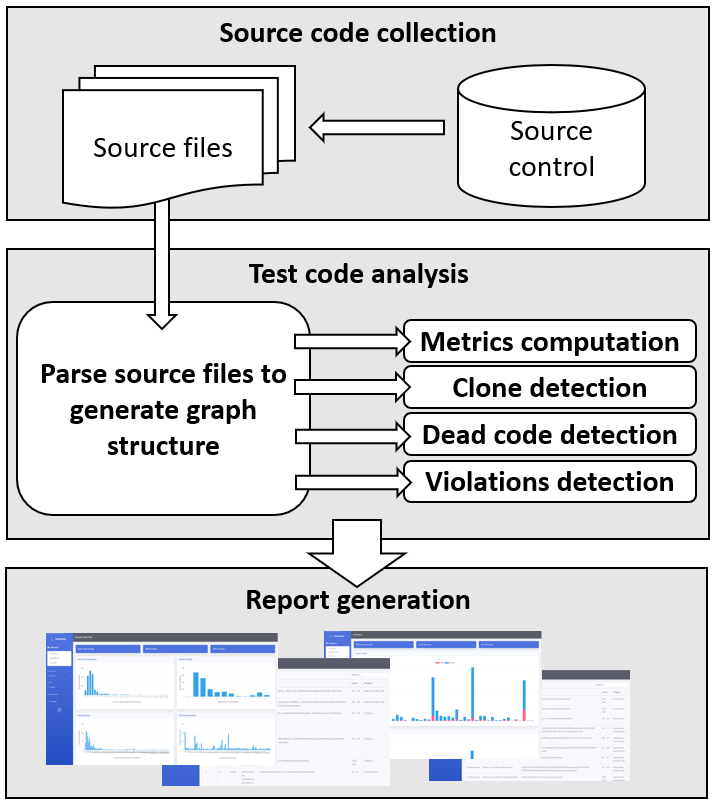
\includegraphics[width=0.5\columnwidth]{figures/ikora/structure.png}
\caption{Main components of \tool}
\label{fig:structure}
\end{figure}

\tool\;\footnote{Availble at \url{https://github.com/UL-SnT-Serval/ikora-inspector}} takes as input the Robot Framework test suites written in the Robot Framework syntax, see \emph{Source code collection} component in Figure~\ref{fig:structure}. Leveraging on the hierarchical structure of the keywords, each test can be represented as an ordered, directed, acyclic $tree\; T$ with nodes $N(T)$ and edges $E(T) \subseteq N(T) \times N(T)$. The nodes $N(T)$ represent keywords and each edge $E(T)$ between two keywords denotes a ``step'': the parent keyword has the child keyword as a \emph{step}. Since keywords can be used multiple times, by more than one tests, the test suite considered as a whole can be represented as a \gls{dag}, $G$, where each node is defined as one of:

 \begin{itemize}
     \item \textbf{Test Cases} Entry point into the graph, called by the framework to be executed. Each test case considered individually is the root of a $tree\; T$.
     \item \textbf{User Keywords} Internal nodes of the graph, they are created by the user, hence their name, to provide modularity and explainability to the test. Each User Keyword is composed of \emph{steps}, which are calls to a User Keyword or to Library Keyword.
     \item \textbf{Library Keywords} Represent the exit point of the graph to perform concrete actions on the \gls{sut}, or the leaves of the tree representation of a single test. Provided by the framework or external libraries, they perform concrete actions, such as interactions with the \gls{sut}, logging or assertions.
 \end{itemize}

\begin{table}[!t]
\def\arraystretch{1.0}
\caption{Clone types}
\label{table:clones}
\centering
\begin{tabular}{>{\raggedright}m{0.5in}>{\raggedright}m{4.4in}}
\toprule
\textbf{\scriptsize{Label}} & \textbf{\scriptsize{Explanation}}\tabularnewline
\toprule

\scriptsize{\textit{Type I}} & \scriptsize{Identical keywords except for changes in whitespace, layout and documentation. The clone detection algorithm tags a keyword pair as Type I clones only in the case of an empty set of differences.}
\tabularnewline

\scriptsize{\textit{Type II}} & \scriptsize{Keywords with a content syntactically identical except for step arguments and return values. The clone detection algorithm tags a pair as Type II clones only if the set contains differences of type \emph{update step arguments} and/or \emph{update step return values}}
\tabularnewline

\scriptsize{\textit{Type III}} & \scriptsize{Superset of Type II clones, ignoring differences of type  \emph{update step}, \emph{add step} and \emph{remove step} if the step belongs to the category \emph{logging}.}
\tabularnewline

\scriptsize{\textit{Type IV}} & \scriptsize{Keyword performing the same sequence of actions on the \gls{sut}, regardless of the internal configuration of the tree. The clone detection algorithm tags a keyword pair as Type IV clones if the sequences of leaf nodes is strictly identical.}
\tabularnewline

\bottomrule
\end{tabular}
\end{table}
    

We use the generated DAG as an intermediate representation of the test code to perform our analysis, see \emph{Test code analysis} component in Figure~\ref{fig:structure}. The tool supports multi projects analysis building a single graph for all the project while annotating each node with the project it belongs to. This representation allows the use of graph theory in order to generate metrics, detect violations, duplicated test code and dead test code. Note that while the tool targets the specific syntax of Robot Framework in this first version, extracting the parsing module would allow to support different syntax for KDT since all analysis are performed on a intermediate representation of the language.

The results of the analysis are presented in a static website composed of a series of dashboards providing information both at the inter- and intra-project level, see \emph{Report generation} component in Figure~\ref{fig:structure}. The content of the dashboards are defined with the help of our partners at \BGL, who are already using the tool in production.

In the remaining of this section, we present the different type of analysis performed on the intermediate representation of the test code base.

\subsection{Projects Dependency Graph}
\label{sec:dependency-graph}

To improve modularity and re-usability testers build generic libraries containing low level functionalities that can be reused by different projects. The \emph{project dependency} module of the tool provides a way to visualize dependencies between projects. The need for this visualization originated from what we consider as weakness of the Robot Framework language, namely, the way transitive dependencies are managed. Unlike popular languages like Java, C++ or Python, when a file is loaded by another one, all its dependencies are loaded and made visible as well.  

\begin{figure}[t!]
\centering
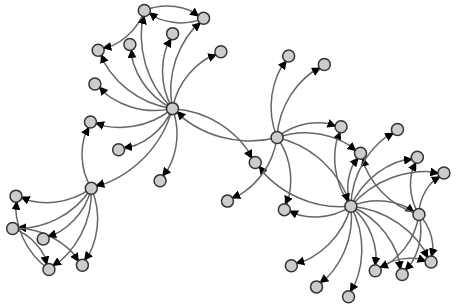
\includegraphics[width=0.5\columnwidth]{figures/ikora/dependency-graph.png}
\caption{Projects Dependency Graph extracted from \tool}
\label{fig:dependency-graph}
\end{figure}

\paragraph{Output} The dependency graph page of the tool presents a complete project dependency graph, allowing the tester to assess the complexity of the test suites as well as detecting issues such as cyclic dependencies. Furthermore, as shown in Figure~\ref{fig:dependency-graph}, the graph can become complex and difficult to analyze, therefore in each project page, we can observe a graph of its dependencies as well as projects depending on it.

\subsection{Project Statistics}

One of the criteria often linked to maintenance effort is the complexity of a project. The more complex a project and its components are, the harder it is to make it evolve and maintain the test code base. Detecting in time the growth of complexity of a project might prevent it from becoming to hard to manage. To this end, we defined a series of four metrics focusing on the complexity of the keywords composing a project.

\subsubsection{Keywords Size} The \emph{size} of keyword $k$ (Test Case or User Keyword), is the number of nodes that exist on the subpath(s) from $k$ to all the leaf keywords (Library Keyword).

\subsubsection{Keywords Level} The \emph{level} of keyword $k$ (Test Case or User Keyword), is the maximum number of edges that exist on the subpath(s) from $k$ to a leaf keyword (Library Keyword). According to the philosophy of \gls{kdt}, the higher the value is, the more abstract the keyword. High-level keywords define business processes while low-level keywords define a concrete way of interacting with the \gls{sut}.

\subsubsection{Keywords Connectivity} The \emph{connectivity} of a keyword is a metric of re-usability among the keywords. Let keyword $k$ belong to a $graph\; G$, then we calculate the connectivity of $k$ by counting the number of nodes (keywords) in the subpath(s) from the entry points of $G$ to $k$.

\subsubsection{Test Cases Sequence Length} Let a test case $TC$ be the root of a $tree\; T$. The \emph{sequence length} of a test case $TC$ is the number of concrete actions performed by the test, defined as the number of leaf nodes of the $tree\; T$.

\subsection{Duplicate Test Code Detection}

\begin{figure}[t!]
\centering
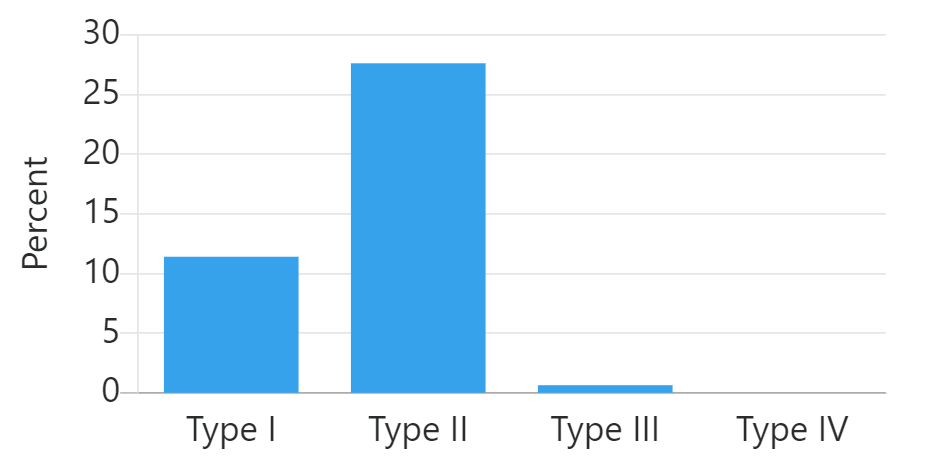
\includegraphics[width=0.75\columnwidth]{figures/ikora/clones.png}
\caption{Percentage of duplicated lines extracted from the Summary Page of \tool}
\label{fig:clones}
\end{figure}

In Chapter~\ref{chap:evolution-system-user-interactive-test}, we observe a large amount of similar test code, \ie\ clones. We observe that clones composed up to 30 percent of the total amount of keywords, indicating that almost one-third of the test code written is duplicated. Clones create several difficulties with inconsistencies during test code evolution generating bugs. Furthermore, we observed that about 50 percent of the strictly similar test code (clone Type I) evolve identically, indicating an added cost in the maintenance cost completely avoidable by refactoring.

The clone detection algorithm is based on the fine-grained changed algorithm defined in Section~\ref{sec:evolution-protocol-rq1} which extracts the changeset between two keywords. The clone detection, ignoring changes impacting the documentation and the name of the keyword, detect the changes between the two keywords and assign a clone category defined in Table~\ref{table:clones} for each pair of keywords. If a pair does not satisfy any of the definitions, then the keywords are not clones.

\paragraph{Output} In the summary, see Figure~\ref{fig:clones}, and in each of the project pages, statistics about the amount of duplicated test code are displayed in order for the tester to evaluate the level of duplication of the test codebase. Furthermore, a test code duplication page offers a table containing all the clones, clustered by groups of similar keywords. Each row contains information about the location of the keywords duplicated, the type of clones, and whether the clones are inter- or intra-application.

\subsection{Dead Test Code Detection}

During refactoring and evolution activities, the call graph might generate keywords not called by any other. In this work, we define dead test code any User Keyword or Variable never called in a \emph{step}, in other words not connected to a Test Case, and therefore never executed. While building the graph representation of the test suite, the tool keeps track of all the callers and the callees for each keyword are variable. Therefore, detecting dead test code only consists of flagging User Keywords and Variables for which no callers were detected. 

\paragraph{Output} For each project, the percentage of dead test code is presented in terms of lines of code, see Figure~\ref{fig:dead-code}. Furthermore, a dead test code page contains a table where each row contains information about the location of the unused User Keywords and Variables in order for the tester to be able to locate them and clean the test code.

\begin{figure}[t!]
\centering
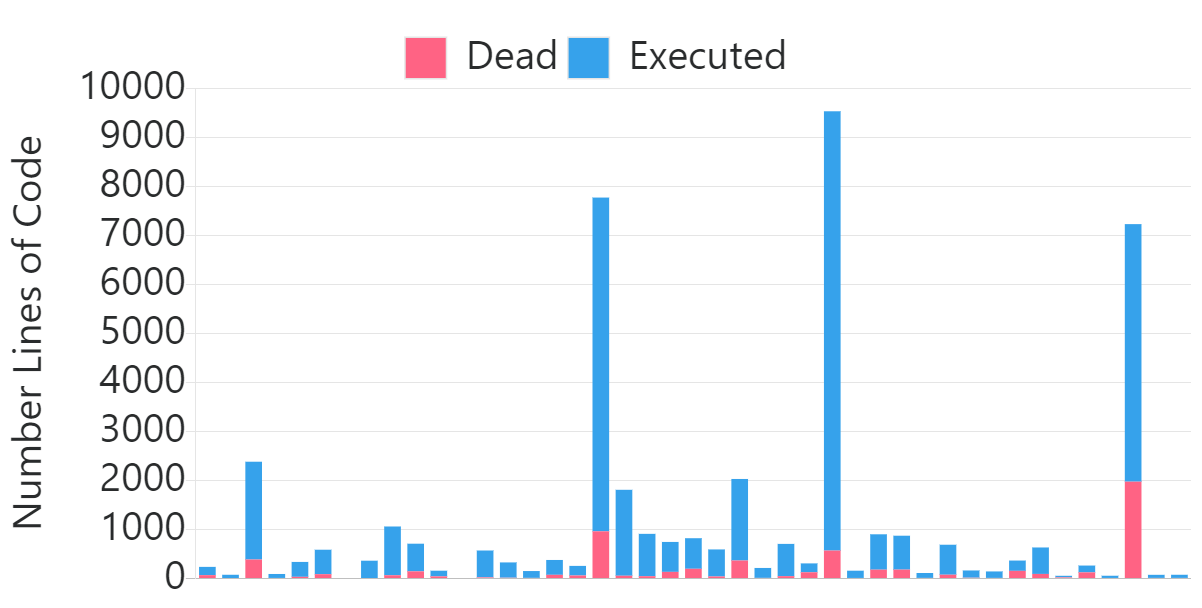
\includegraphics[width=0.75\columnwidth]{figures/ikora/dead-code.png}
\caption{Number of lines of dead test code per project extracted from the Summary Page of \tool}
\label{fig:dead-code}
\end{figure}

\subsection{Bad Practices and Error Detection}

In its current version the tool allows to detect two types of bad practices specific to Robot Framework, 16 smells common to \gls{suit} and two error types. However, conducting an analysis of the typical change patterns and the execution results, we intend to extend the set, specifically to address issues such as weak \emph{locators} and weak \emph{synchronization} points causing false positive and flakiness.

\subsubsection{Duplicated Keyword Error} If two keywords have the same name in the same scope, it causes the program to crash during runtime. However, since keyword resolution is a dynamic process in Robot Framework, the error might be revealed after a long execution time, reducing the velocity of the team to detect and address such bugs. During the analysis, while resolving names, the tool checks for duplicate names.

\subsubsection{Missing Definition} Identifies \emph{steps} for which no keyword is associated or a missing variable, therefore generating an edge in the graph with no target node. Upon analysis of the results, we observe that we have false positives for keywords generated dynamically and therefore invisible during static analysis. This violation constitutes the only one generating false positive, however, relying too heavily on dynamic loading might hinder the readability of the test suite and therefore, the results are kept and displayed.

\subsubsection{Transitive Dependency Warning} We call transitive dependency warning a call to a keyword not defined in the same file or in a direct dependency but in an indirect dependency as explained in Section~\ref{sec:dependency-graph}.

\subsubsection{Duplicated Variable Warning} During the resolution of variable names, if two variables have the same name and are defined in \emph{Variable} blocks, the framework loads the first variable it encounters and discards all subsequent definitions. This behavior might lead to unexpected behavior, assigning wrong values to variables.

\subsubsection{SUIT Smells} Relying on the tooling introduced in Chapter~\ref{chap:smells-system-user-interactive-test}, \tool\ is able to detect the number of symptoms present in a test. Relying on rules inserted by the user, whenever this number is exceeded, the test case is flagged as smelly. Because the nature of \tool\ is to offer an overview of the project, the detection of symptoms for SUIT smells is also available as a SonarQube Plugin\footnote{Available at \url{https://github.com/kabinja/sonar-ikora-plugin}}

\paragraph{Output} All these errors and warnings are grouped in a single table, giving the level of the violation (warning or error) as well as the location and its reason. Each row of the table contains information about the location of the violation, the cause, and its severity.
